
\textbf{Ejemplo 1}\\
Una persona invierte 600{.}000  COP en un depósito a término fijo en 6 meses,a una tasa 24\%
nominal anual mes vencido, determinar la tasa efectiva anual y el valor del documento
suponiendo una retención en la fuente sobre utilidades del 7\%.\\ \\
%\newpage %USAR SOLO SI EL SOLUCIÓN QUEDA SOLO Y ES NECESARIO BAJARLO A LA SIGUIENTE PAGINA
\textbf{Solución.}\\
%La tabla ira centrada
\begin{center}
 \renewcommand{\arraystretch}{1.5}% Margenes de las celdas
 %Creación de la cuadricula de 3 columnas
 \begin{longtable}[H]{|c|c|c|}
  %Creamos una linea horizontal
  \hline
  \multicolumn{3}{|c|}{\cellcolor[HTML]{FFB183}\textbf{1. Asignación de periodo focal}}                                                                                                                \\ \hline
  \multicolumn{3}{|c|}{$pf = 6 \hspace{1mm} pmv$}                                                                                                                                      \\ \hline

  %Definimos el color de la primera fila
  \rowcolor[HTML]{FFB183}
  %%%%% INICIO DECLARACIÓN DE VARIABLES %%%%%%%
  %%%%%%%%%% INICIO TITULO
  %Lo que se hace aquí es mezclar las 3 columnas en una sola
  \multicolumn{3}{|c|}{\cellcolor[HTML]{FFB183}\textbf{2. Declaración de variables}}                                                                                                   \\ \hline
  %%%%%%%%%% FIN TITULO
  %%%%%%%%%% INICIO DE MATEMÁTICAS
  %Cada & hace referencia al paso de la siguiente columna
  $P =  600{.}000\ COP$                                                             & $m_{1} = 12 \textit{ pmv} $                                             & $F =  ? COP $                  \\
  $i= 2\% \textit{ pmv}$                                                       & $m_{2} = 1 \textit{ pmv} $                                              & $j_{2} = ?\% \textit{ naav} $ \\
  $n = 6  \textit{ pmv}  $                                                     & $j_ {1} = 24\% \textit{ namv} $                                         &                             \\
  $RF = 7\% \textit{ Retencion en la fuente}$                                  &                                                                         &                             \\\hline

  %%%%%%%%%% FIN DE MATEMÁTICAS
  %%%%% FIN DECLARACIÓN DE VARIABLES


  %%%%% INICIO FLUJO DE CAJA
  \rowcolor[HTML]{FFB183}
  \multicolumn{3}{|c|}{\cellcolor[HTML]{FFB183}\textbf{3. Diagrama de flujo de caja}}                                                                                                  \\ \hline
  %Mezclamos 3 columnas y pondremos el dibujo
  %%%%%%%%%%%%% INSERCIÓN DE LA IMAGEN
  %Deberán descargar las imágenes respectivas del drive y pegarlas en la carpeta
  %n_capitulo/img/ejemplos/1/capitulo1ejemplo1.pdf  (el /1/ es el numero del ejemplo)
  \multicolumn{3}{|c|}{ 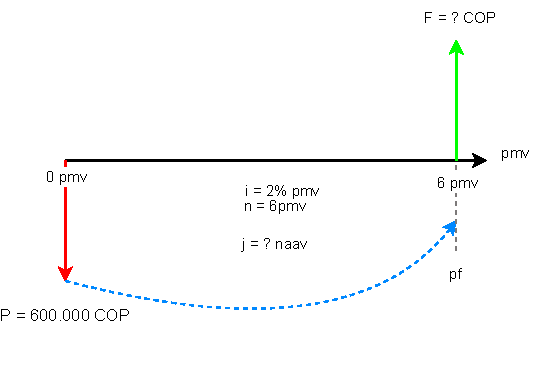
\includegraphics[trim=-78 -5 -78 -5]{3_Capitulo/img/ejemplos/1/capitulo3ejercicio1.pdf} }                                                                                      \\ \hline
  %%%%%%%%%%%%% FIN INSERCIÓN DE IMAGEN
  %%%%%FIN FLUJO DE CAJA



  %%%%% INICIO DECLARACIÓN FORMULAS
  %%%%%%%%%%% INICIO TITULO
  \rowcolor[HTML]{FFB183}
  \multicolumn{3}{|c|}{\cellcolor[HTML]{FFB183}\textbf{4. Declaración de Fórmulas}}                                                                                                    \\ \hline
  %%%%%%%%%%% FIN TITULO
  %%%%%%%%%%% INICIO MATEMÁTICAS

  $F = P(1+i)^n \hspace{0.3cm} \textit{Valor futuro}$                          & \multicolumn{2}{c|}{$(1+i_{1})^{m_{1}}=(1+i_{2})^{m_{2}}$  \textit{equivalencia de tasas}}                                            \\
  $j = i \cdot m \hspace{0.3cm} \textit{Tasa de interés periodica anualizada}$ & \multicolumn{2}{c|}{$I=F-P \hspace{0.3cm} \textit{Valor futuro neto}$}                                \\ \hline
  %%%%%%%%%% FIN MATEMÁTICAS
  %%%%%% INICIO DESARROLLO MATEMÁTICO
  \rowcolor[HTML]{FFB183}
  %%%%%%%%%%INICIO TITULO
  \multicolumn{3}{|c|}{\cellcolor[HTML]{FFB183}\textbf{5. Desarrollo Matemático}}                                                                                                      \\ \hline
  %%%%%%%%%% FIN TITULO
  %%%%%%%%%% INICIO MATEMÁTICAS
  $(1 + 0,02)^{12}= (1 + i_{2})^{1}$                                           & \multicolumn{2}{|c|}{$F =   600{.}000 \ COP \ (1+0,02)^6$}                                                     \\
  $i_{2}=(1+0,02)^{12}-1=0,26824179$                                           & \multicolumn{2}{|c|}{$F =  675{.}697,45 \ COP $}                                                            \\
  $j_{2}=0,26824179 \cdot 1 = 0,26824179\%naav$                                  & \multicolumn{2}{|c|}{$I = | F - P | = |   675.697,45 \ COP-  600.000 \ COP|$}                                  \\
  $j_{2}=26,824179\% \textit{ naav}$                                             & \multicolumn{2}{|c|}{$I = | F - P | = |  75.697,45  \ COP |$}                                               \\
  $j_{2}=26,48\% \cdot 1 = 26,48\% \textit{naav}$                                & \multicolumn{2}{|c|}{$RF = 0,07 \cdot  75{.}697,45 \ COP =  5{.}298,82 \ COP$}                                    \\
                                                                               & \multicolumn{2}{|c|}{$F_{final} =   675{.}697 \ COP-  5{.}299 \ COP =   670{.}398 \ COP$}                               \\ \hline


  %%%%%%%%%% FIN MATEMÁTICAS
  %%%%%% FIN DESARROLLO MATEMÁTICO
  %%%%%% INICIO RESPUESTA
  \rowcolor[HTML]{FFB183}
  %%%%%%%%%%INICIO TITULO
  \multicolumn{3}{|c|}{\cellcolor[HTML]{FFB183}\textbf{6. Respuesta}}                                                                                                                  \\ \hline
  %%%%%%%%%% FIN TITULO
  %%%%%%%%%% INICIO RESPUESTA MATEMÁTICA
  \multicolumn{3}{|p{\textwidth}|}{
  El valor del documento después de impuestos es de $ 670{.}398 \ COP$ que es menor que $F =  675{.}697,45 \ COP$ y obviamente se reduce la tasa de nominal anual mes vencido $j = 24,84\% \textit{ naav}$ .
  }                                                                                                                                                                                    \\ \hline


  %%%%%%%%%% FIN MATEMÁTICAS
  %%%%%% FIN RESPUESTA
 \end{longtable}
 %Se crean dos lineas en blanco para que no quede el siguiente texto tan pegado
 %\newline \newline %USARLO SI CREES QUE ES NECESARIO
\end{center}